\begin{comment}
\section*{Endocrine Control}
 \textrightarrow~ discuss the underlying problem an animal body faces to control its interior environment,
	 \begin{itemize}
	  \item anatomical figurines and students shall discuss (in pairs) how the organs could be controled; think about quick and short vs slow and longterm
	  \item discuss diff. concepts: neural signalling vs chemicals in the blood stream
	  \item BB-sketch: cell - bloodstream - cell (like biozone human p.93)
	  \item chemicals in the blood = hormones \textrightarrow~ how can they act at the target?
	 \end{itemize}

\begin{figure}[h]
 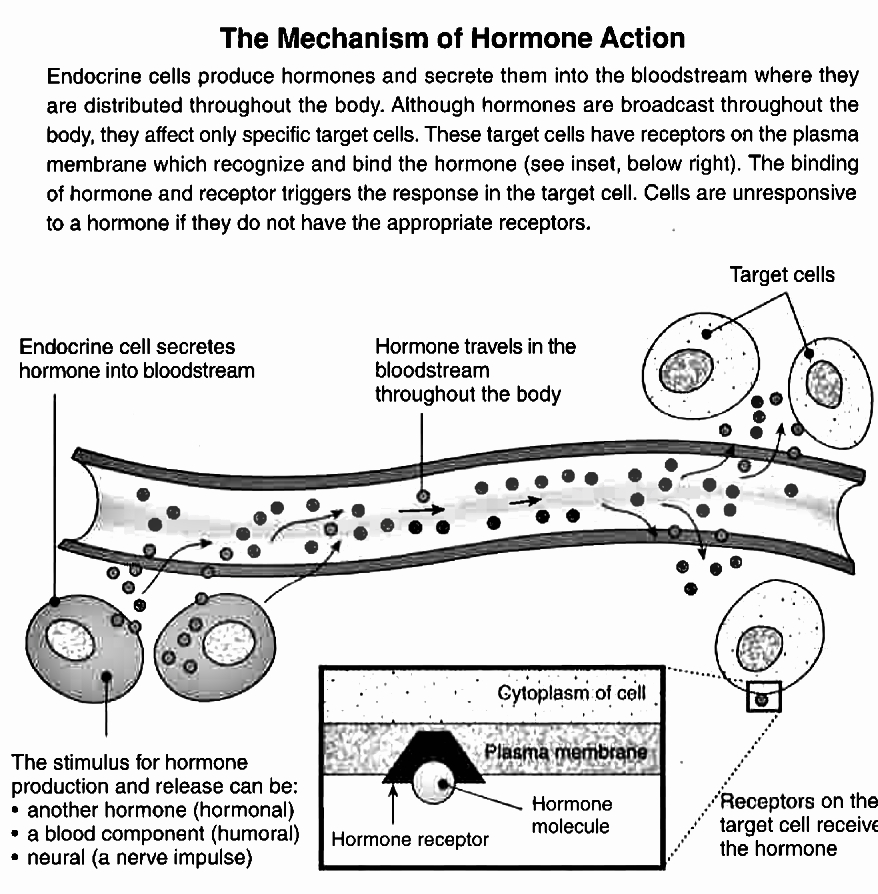
\includegraphics[width=6cm]{/images/biozone-human-0093_v1.jpg}
\end{figure}

	 
	 
Overview Endocrine System: label the figure
 \newpage
 ...empty page...
\newpage \addtocounter{page}{-2}
\end{comment}


\section{Endocrine Control} \label{sec:EndocrineControl}
 
		\begin{mdframed}[style=exampledefault, userdefinedwidth=15cm, frametitle={Starr 31.1}\label{mat:BEISPIELMATERIAL}]	  
			Starr covers the topic of \emph{endocrine control} excellently in chapter 31, starting on p. 535. The following sub-chapters are part of our syllabus: 31 (p.535), 31.1, 31.2, 31.3, 31.4, 31.5, 31.6, 31.7 31.8 (.\textit{.. virtually the entire chapter...})
		\end{mdframed}

\begin{enumerate}[resume, leftmargin=*]
\item  Identify the endocrine organs shown in figure \ref{fig:EndokrinSystem}, label them and write a short description to each of these organs and their functions! \\ \emph{Also highlight every organ and its function-description in a specific colour!} 
\end{enumerate}


 \enlargethispage{2cm}
% \hspace{-2cm}
\Ersatz{
	\begin{minipage}{15cm}
	   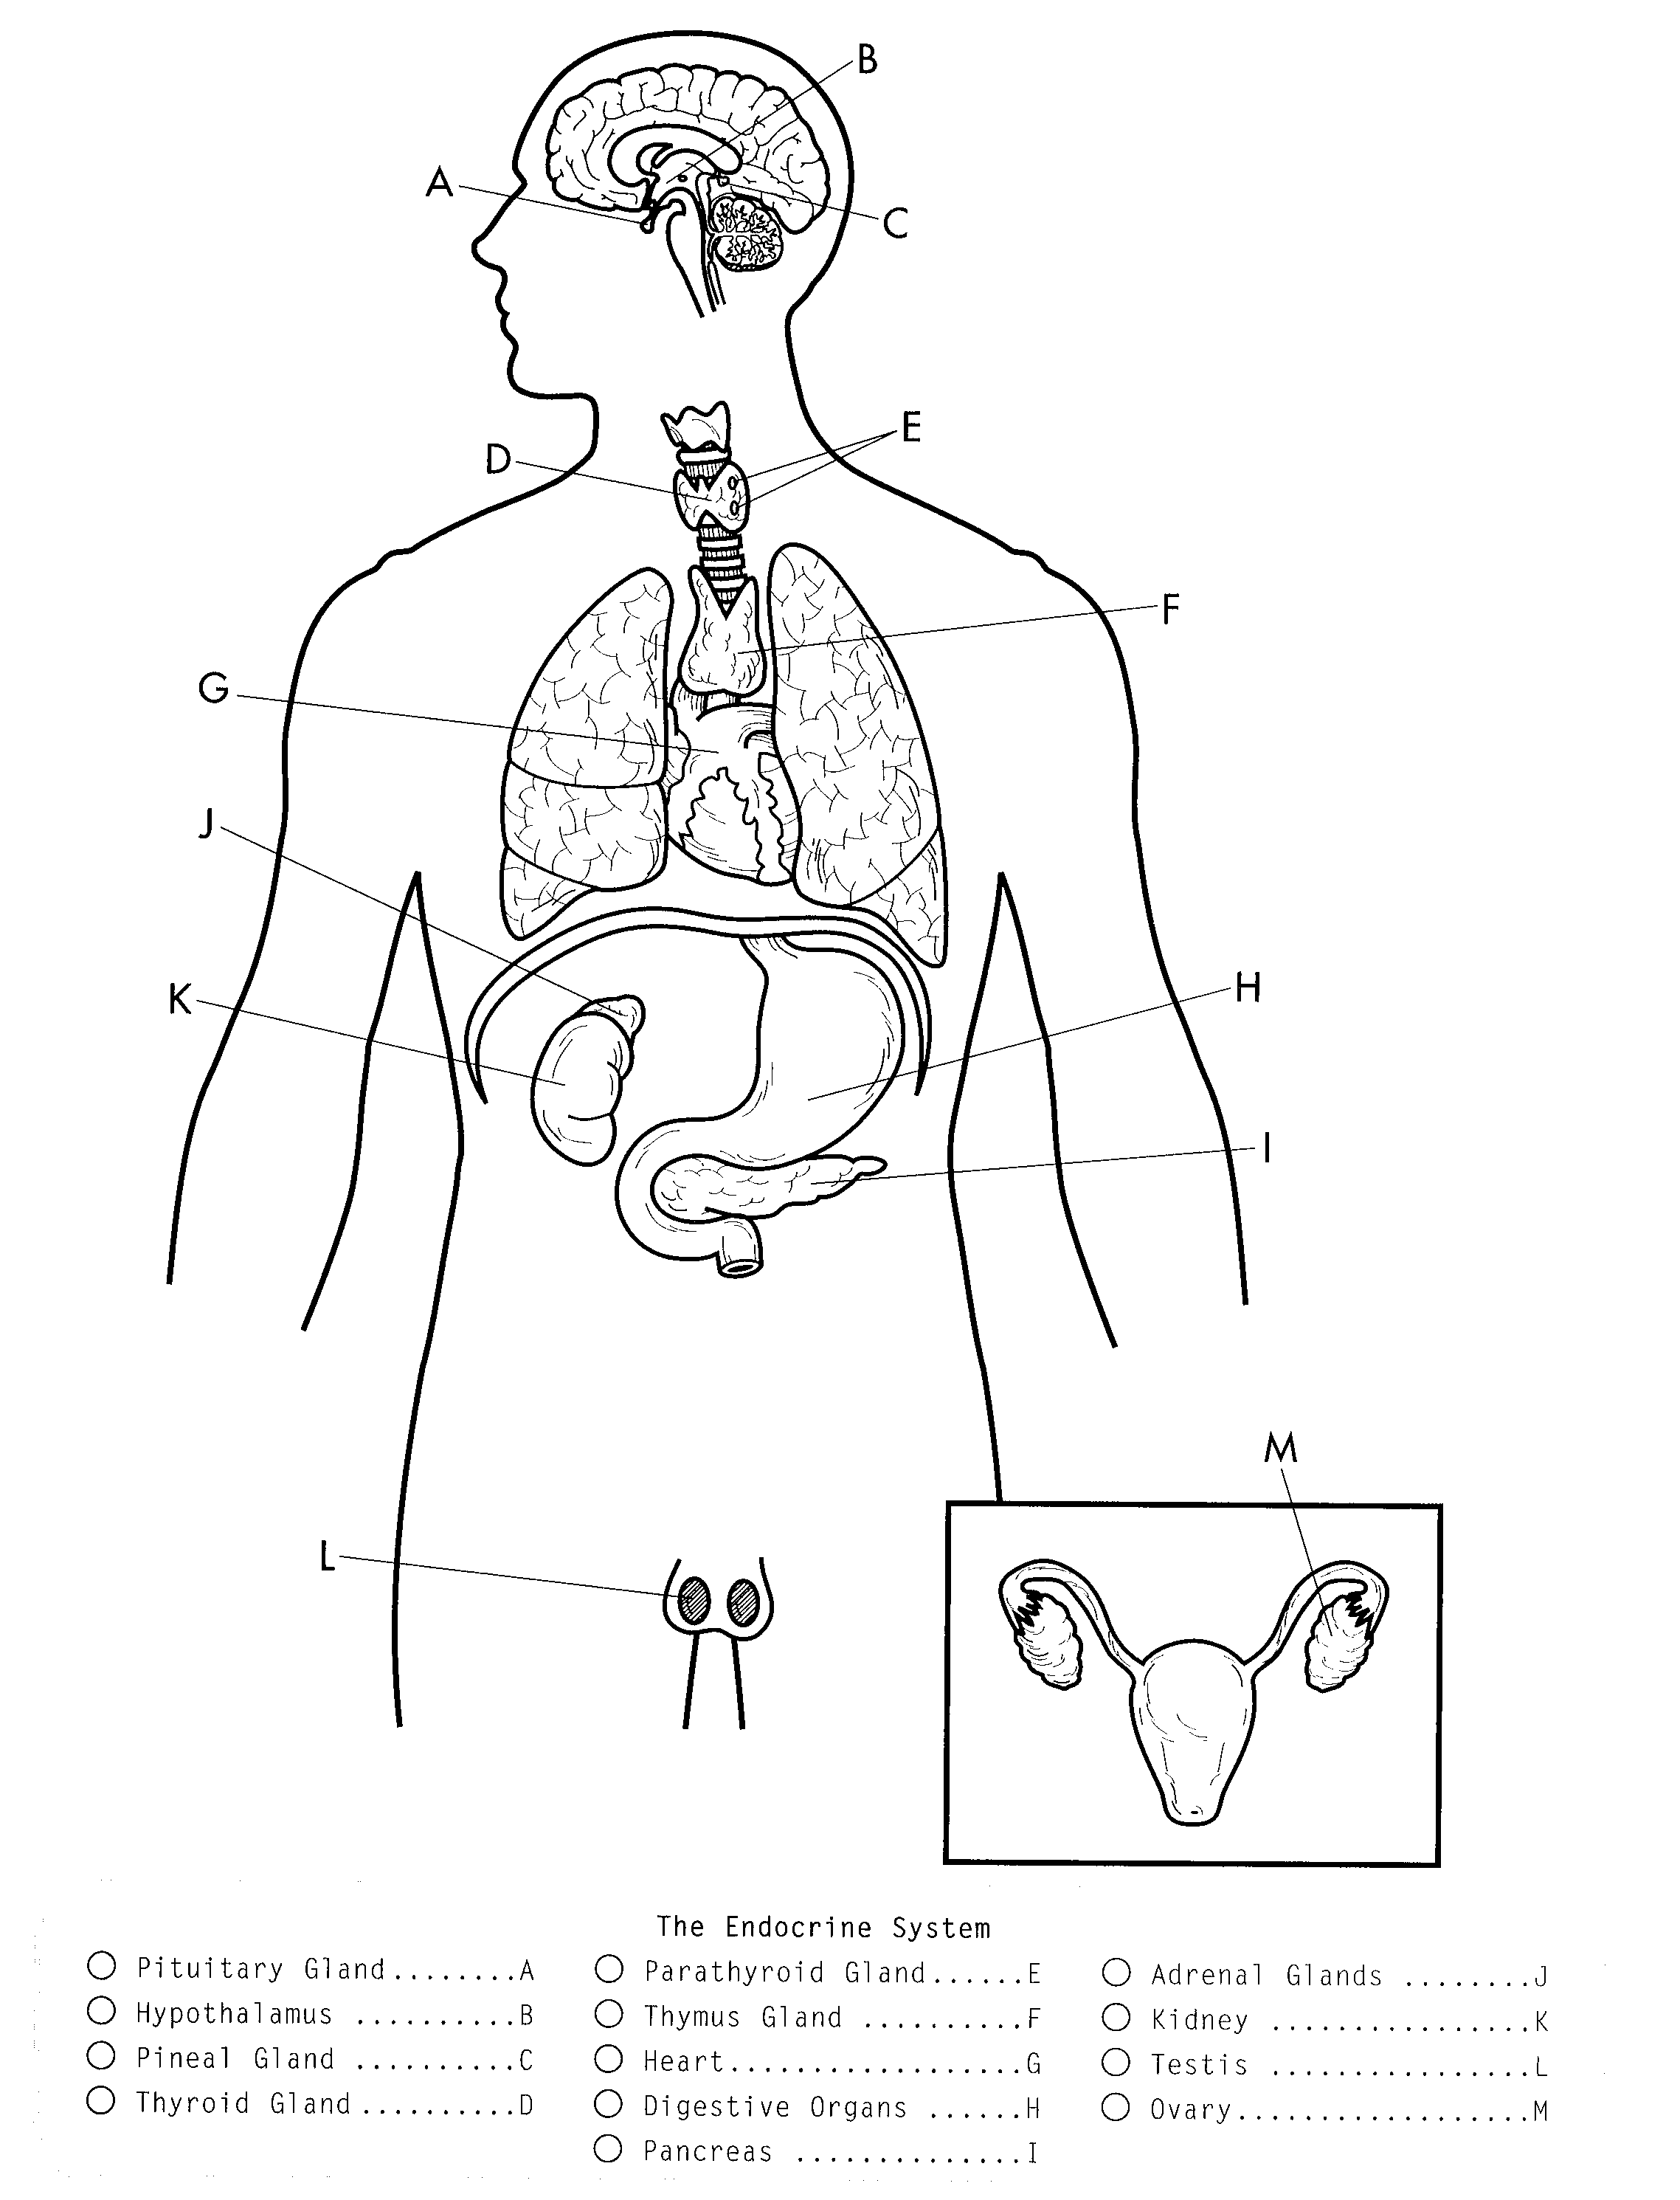
\includegraphics[width=0.95\textwidth]{/images/BiolColBook_245_v2.png} 
	 \captionof{figure}[Endokrines System aus dem Biology Coloring Book]{The human endocrine system:   hormone producing organs.}
			      \label{fig:EndokrinSystem}
	\end{minipage}
	}{%%
		\begin{minipage}{15cm}
	   \includegraphics[width=0.95\textwidth]{/images/BiolColBook_245_v3.png} 
	 \captionof{figure}[Endokrines System aus dem Biology Coloring Book]{The human endocrine system:   hormone producing organs.}
			      \label{fig:EndokrinSystem}
	\end{minipage}
	}



\clearpage
\subsubsection{There are two ways a hormone may act}\label{sss:HormonesActDifferent}
Hormones may have different effects and response times 
				 \marginline{\textrightarrow~\texttt{ in all cases hormones are transported by the blood stream. How manages your body to react so different to the presence of a hormone?} \textleftarrow~}
\begin{itemize}
 \item Adrenalin, a very quick acting hormone: \hrefL{/temp/temp-filme/Best of Summer 2012 - Adrenalin Junkies-3qd37C9aLZ8.mp4}{https://www.youtube.com/watch?v=3qd37C9aLZ8}{Adrenalin Junkies (youtube)}
 \item Insulin, a hormone that acts quite fast and if absent, may be added
 artificially: \hrefL{/temp/temp-filme/A Day in the Life of Diabetes-bHyPWkWjAkM.mp4}{https://www.youtube.com/watch?v=bHyPWkWjAkM}{A day in the life of two girls (4, 11) with diabetes (youtube)}
 \item Sexual hormones such as estrogen, progesteron or testosteron act very slow and show their effects over years: \hrefL{/temp/temp-filme/Puberty - The Infographics Show-TRyOcLSJDzk.mp4}{https://www.youtube.com/watch?v=TRyOcLSJDzk}{Effects of sexual hormones during puberty (youtube)}
 \item The signal molecules or enzymes released by the effector cells alter growth, behaviour or physical reactions of the body.
\end{itemize}



% \subsubsection{Paracrine, endocrine, autocrine}
% 
% \todo[inline]{fig. from biozone p.94 -- erase the paths of the hormones: HP work}


\subsubsection{Signal transduction}
\hspace{-2cm}
\enlargethispage{3.4cm} \thispagestyle{plain}
% 	\begin{addmargin*}[-5cm]{-5cm}
	\Ersatz{
		\begin{minipage}{18cm}
		 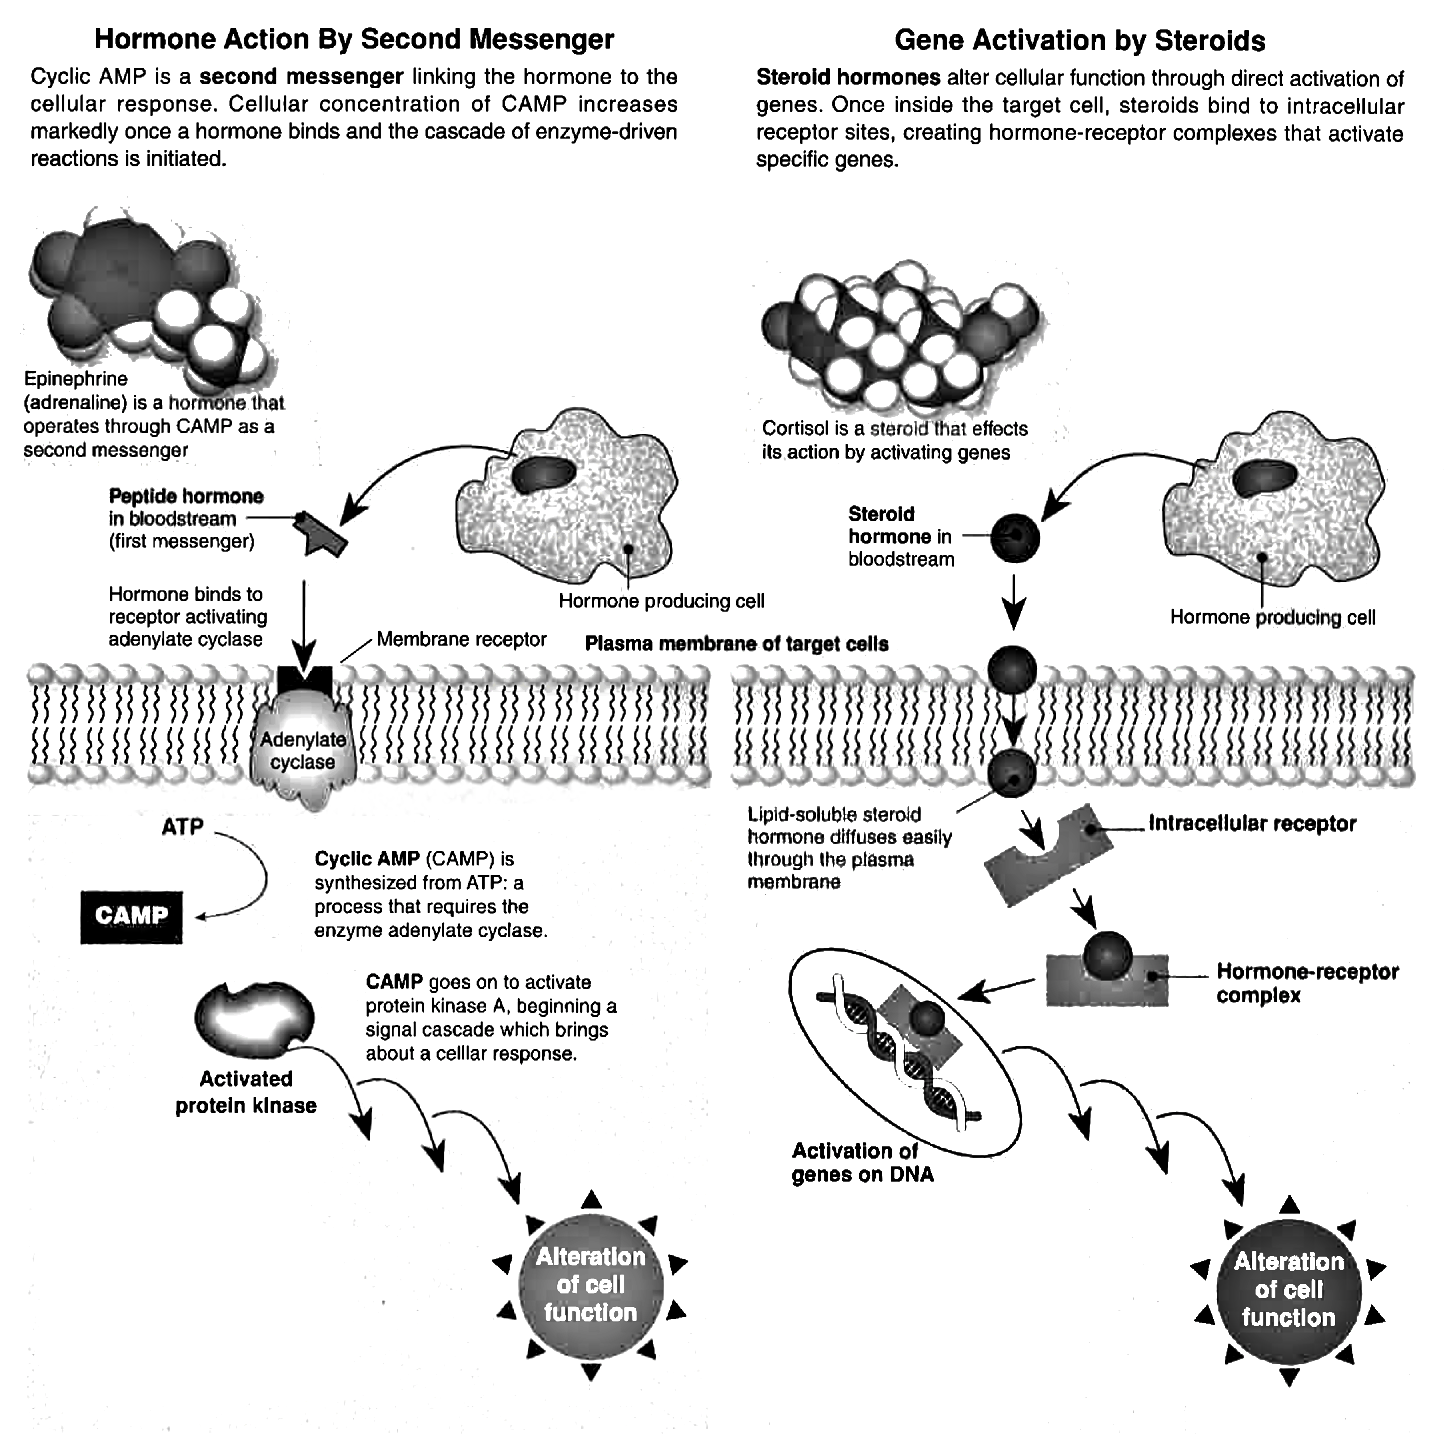
\includegraphics[width=18cm]{/images/biozone-human-0095-1_v2.png}
		 \captionof{figure}[hormones, signal transduction, biozone human p.95]{Two different modes of signal transduction for hormones. Complete these charts using Starr 31.1 (9ed)}
			\end{minipage}
		}{
		\begin{minipage}{18cm}
		 \includegraphics[width=18cm]{/images/biozone-human-0095-1_v5.png}
			  \captionof{figure}[hormones, signal transduction, biozone human p.95]{Two different modes of signal transduction for hormones. Complete these charts using Starr 31.1 (9ed)}
			\end{minipage}
			}

% 	\end{addmargin*}
\clearpage

	
\subsubsection{A déjà-vu: Control of the menstrual cycle}
In grade 3.2 we discussed the development of chordata (\textit{animals with spinal chord}). This was the first time you encountered the effects of hormones. Starr's chapter 31.7 briefly outlines this topic. In figure \ref{fig:MenstrualCycle} some terms have been replaced by \ldots $\leftrightarrow$ please complete these gaps!


	\begin{addmargin*}[-1cm]{-1cm}
	\Ersatz{
		\begin{minipage}{18cm}
		 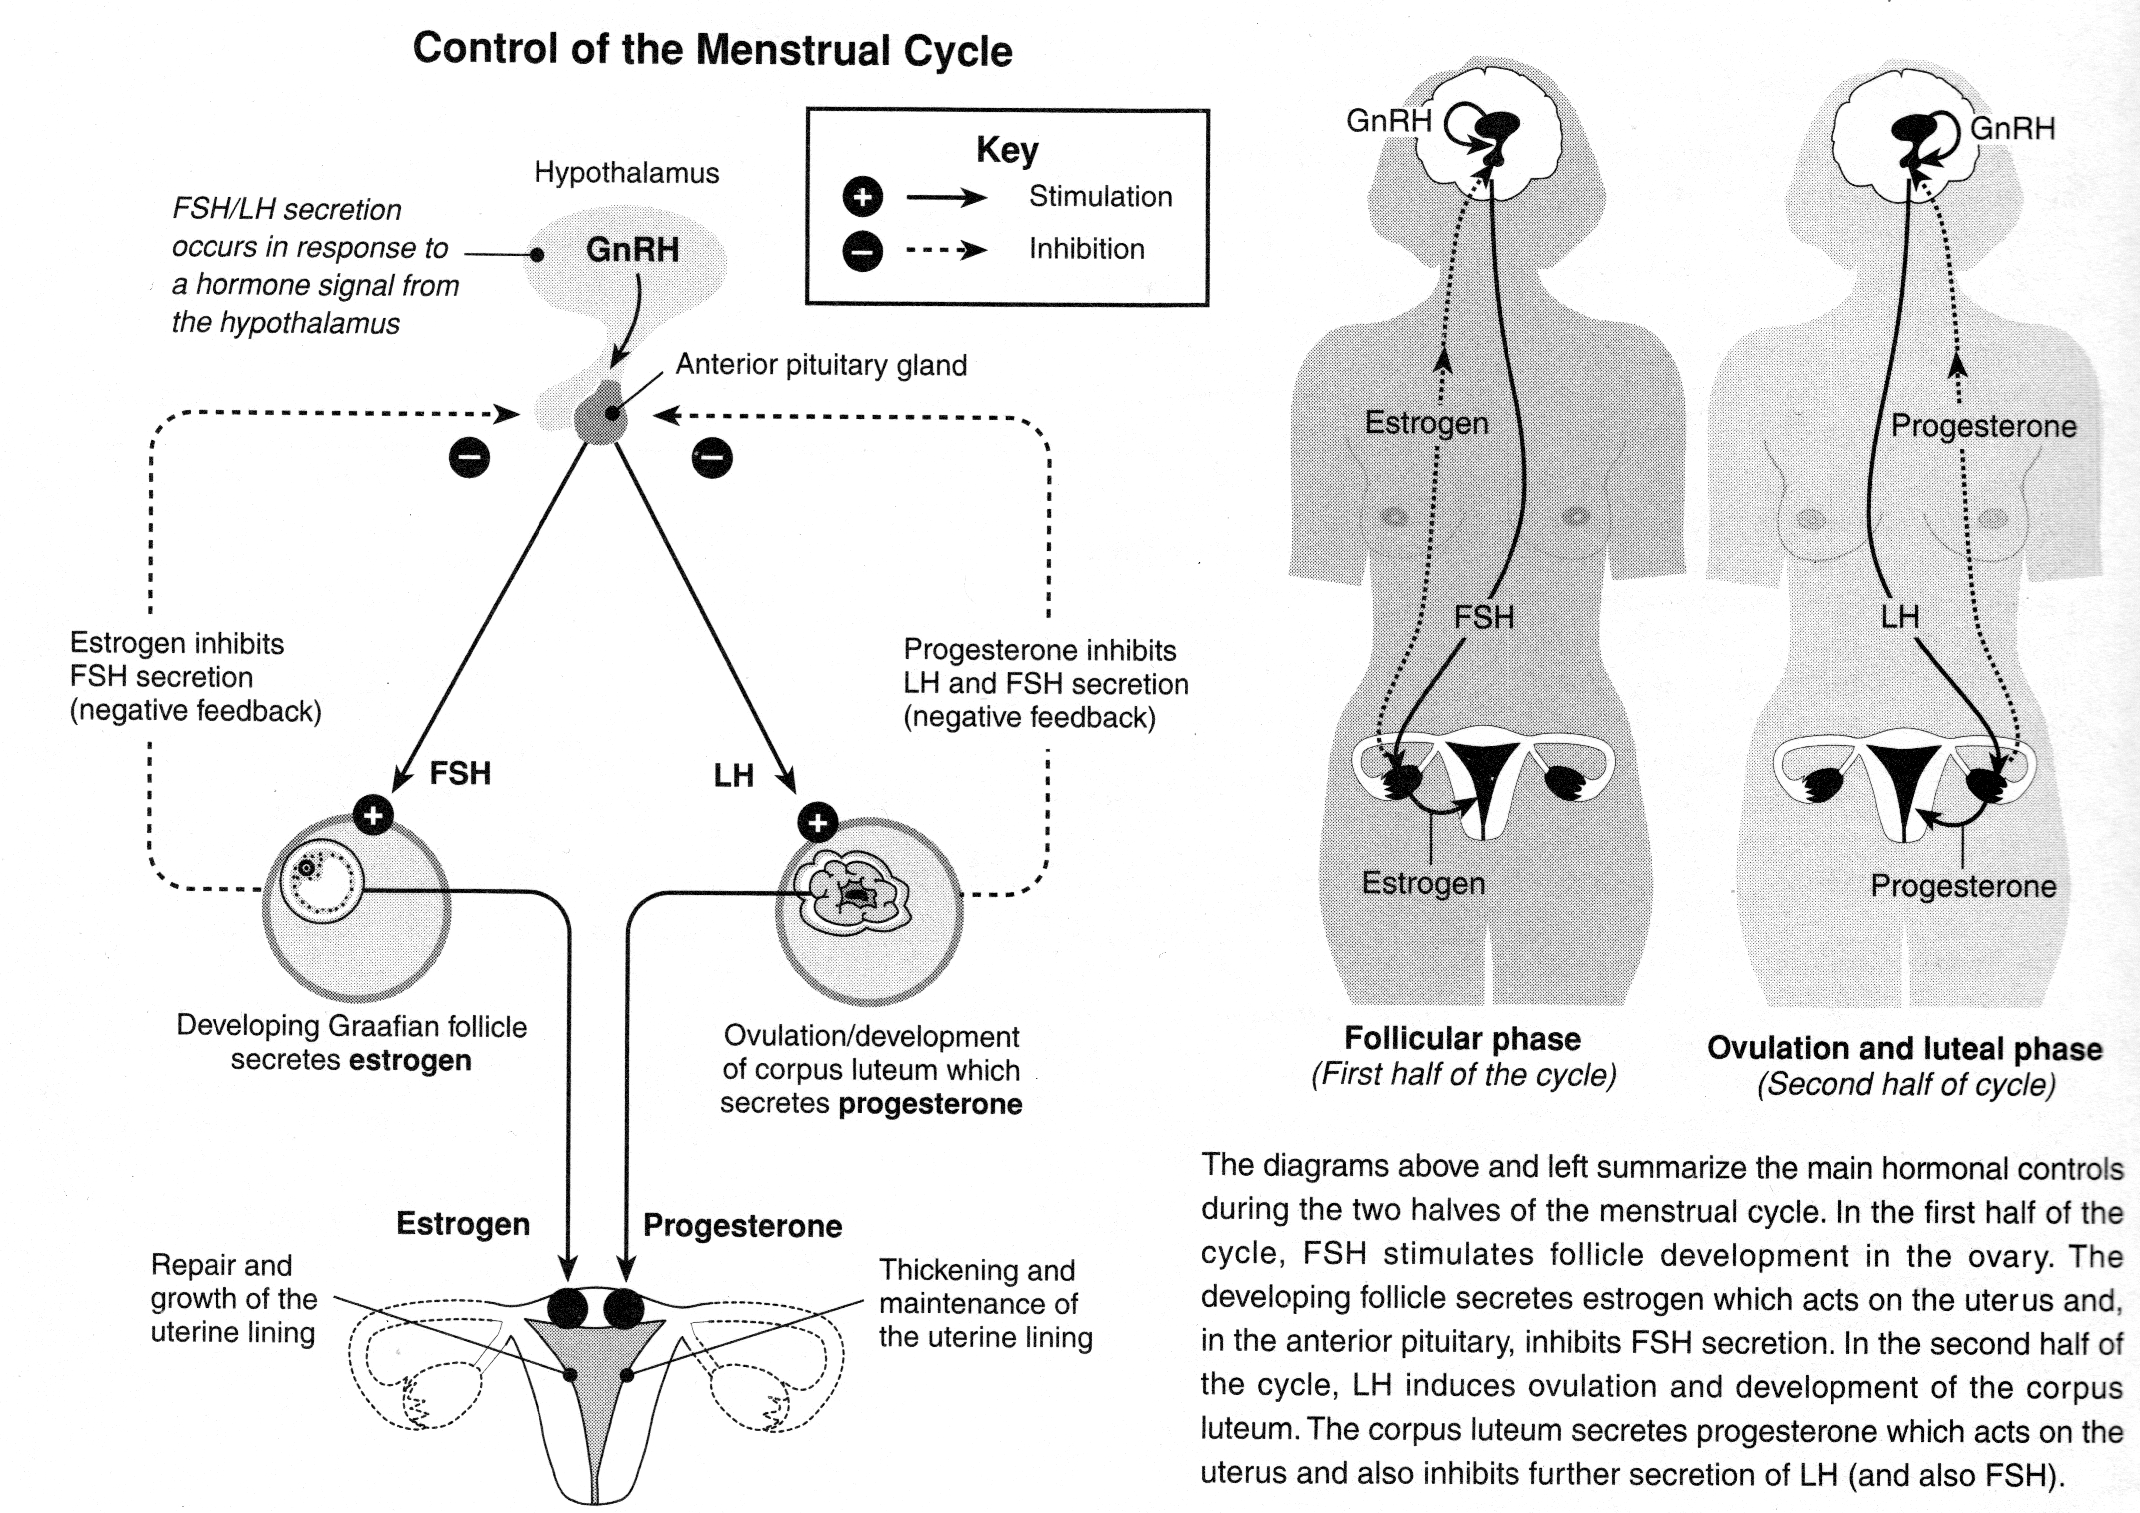
\includegraphics[width=18cm]{/images/biozone-human-0214-o_v1.jpg}
		 \captionof{figure}[regulation of the female menstrual cycle, biozone human p.214]{Hormonal regulation of the female menstrual cycle - add the missing terms!}
		 \label{fig:MenstrualCycle}
			\end{minipage}
		}{
		\begin{minipage}{18cm}
		 \includegraphics[width=18cm]{/images/biozone-human-0214-o_v2.png}
			 \captionof{figure}[regulation of the female menstrual cycle, biozone human p.214]{Hormonal regulation of the female menstrual cycle - add the missing terms!}
		 \label{fig:MenstrualCycle}
			\end{minipage}
			}

	\end{addmargin*}


\fillwithdottedlines{\stretch{1}}
\clearpage
